\section{}
% The installation of a magnetic resonance imaging (MRI) system requires the machine to be well 
% isolated from vibration. The original isolation is shown where the support motion 𝑦 = 𝑌𝑠𝑖𝑛(𝜔𝑡)
% is due to the floor vibrating from the equipment in the room below. This equipment is assumed to 
% run at 2400 rpm, and the natural frequency of the installation is estimated to be 15 Hz.

\textit{The installation of a magnetic resonance imaging (MRI) system requires the machine to be well isolated from vibration. The original isolation is shown where the support motion $y = Y_{sin}(\omega t)$ is due to the floor vibrating from the equipment in the room below. This equipment is assumed to run at 2400 rpm, and the natural frequency of the installation is estimated to be 15 Hz.}

\begin{figure}[H]
    \centering
    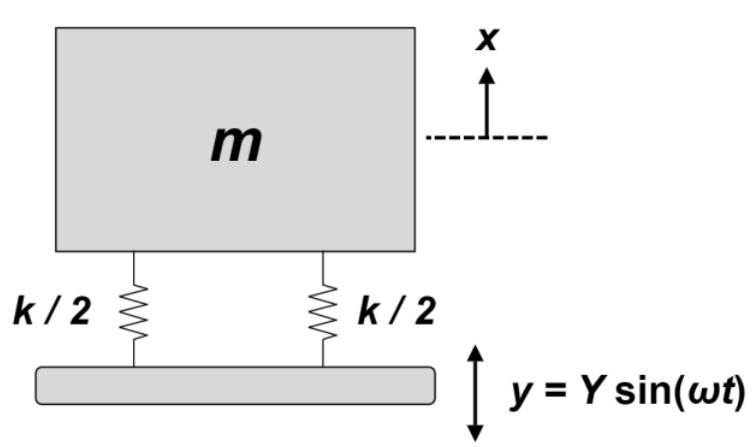
\includegraphics[width=0.5\textwidth]{Questions/Figures/Q2 Problem Diagram.png}
    \caption{MRI system.}
    \label{fig:Q2}
\end{figure}

% (1 pt) Estimate the amplitude of vibration of 𝑚 compared to the amplitude of the floor 
% motion.

\subsection{}
\textit{Estimate the amplitude of vibration of $m$ compared to the amplitude of the floor motion.}

This is a base excitation problem. The frequency is $\omega = \frac{2400}{60} = 40$ Hz. The natural frequency was given as $p = 15$ Hz.
The amplitude compared to the floor motion is 
\begin{align*}
    \frac{\mathbb{X}}{a} &= \frac{\sqrt{1 + \left(2 \zeta \frac{\omega}{p}\right)^2}}{\sqrt{\left[1 - \left(\frac{\omega}{p}\right)^2\right]^2 + \left(2\zeta\frac{\omega}{p}\right)^2}} \\
    &= \frac{\sqrt{1 + \left(2 \cdot 0 \cdot \frac{40}{15}\right)^2}}{\sqrt{\left[1 - \left(\frac{40}{15}\right)^2\right]^2 + \left(2 \cdot 0 \cdot \frac{40}{15}\right)^2}} \\
    &= \boxed{0.1636}
\end{align*}

% (2 pts) As the calculation in (a) indicated that the motion of 𝑚 was too large, the supplier 
% suggests the installation of a damper to give a damping ratio of 𝜁 = 0.2. Will the damper 
% reduce of increase the amplitude of motion? Calculate the difference the damper will make.

\subsection{}
\textit{As the calculation in (a) indicated that the motion of $m$ was too large, the supplier suggests the installation of a damper to give a damping ratio of $\zeta = 0.2$. Will the damper reduce of increase the amplitude of motion? Calculate the difference the damper will make.}

Since the machine is operating above resonance, the effects of damping should increase the amplitude of motion. To confirm this, we can apply the same equation as in part (a) with $\zeta = 0.2$.
\begin{align*}
    \frac{\mathbb{X}}{a} &= \frac{\sqrt{1 + \left(2 \zeta \frac{\omega}{p}\right)^2}}{\sqrt{\left[1 - \left(\frac{\omega}{p}\right)^2\right]^2 + \left(2\zeta\frac{\omega}{p}\right)^2}} \\
    &= \frac{\sqrt{1 + \left(2 \cdot 0.2 \cdot \frac{40}{15}\right)^2}}{\sqrt{\left[1 - \left(\frac{40}{15}\right)^2\right]^2 + \left(2\cdot 0.2 \cdot \frac{40}{15}\right)^2}} \\
    &= \boxed{0.2357}
\end{align*}

\subsection{}
\textit{Another alternative is suggested by a trainee engineer who argued that the machine should be supported from above as well as from the vibration floor as illustrated (it is assumed that the upper support is fixed). Starting from a free body diagram, determine the equation of motion and an expression for the steady state amplitude of $m$. Compare the amplitude of motion of $m$ for this case to the original design in (a) and the alternative design with the damper in (b).}

\begin{figure}[H]
    \centering
    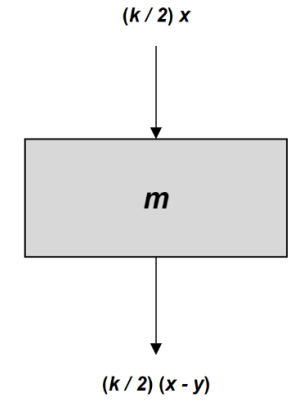
\includegraphics[width=0.5\textwidth]{Questions/Figures/Q2 c).png}
    \caption{MRI system with upper support.}
    \label{fig:Q2 c}
\end{figure}

The equation of motion is then,
\begin{align*}
    \uparrow \sum F_y :&= m \ddot{x} \\
    &= -\frac{k}{2} x - \frac{k}{x} (x - y)
\end{align*}
Then the equation of motion is then,
\begin{align*}
    m \ddot{x} + kx &= \frac{k}{2} y \\
    m \ddot{x} + kx &= \underbrace{\frac{k}{2} Y}_{F_0} \sin(\omega t)
\end{align*}
Which has the amplitude, 
\begin{align}
    \mathbb{X} &= \frac{F_0/k}{\bigg|1 - \left(\frac{\omega}{p}\right)^2\bigg|} \\
    \implies \frac{\mathbb{X}}{a} &= \frac{\frac{1}{2}}{\bigg|1 - \left(\frac{40}{15}\right)^2\bigg|} \\
    &= \boxed{0.0818}
\end{align}

\subsection{}
\textit{Another way to reduce the motion of $m$ is to use a vibration absorber on the original design.}
\textit{i) If the absorber has a mass $m_2$ equal to 15\% of the main mass $m$, calculate the amplitude of motion of the absorber mass at the operating speed (2400 rpm).}
The natural frequency of the large mass in isolation is known,
\begin{align*}
    p_{11} &= \sqrt{\frac{k}{m}} = 15 \text{ Hz}
\end{align*}
To reduce vibrations, select the natural frequency of the absorber mass to be $p_{22} = \omega = 40$ Hz. The amplitude of motion of the absorber mass is then,
\begin{align*}
    \frac{\mathbb{X}_2}{\mathbb{X}_0} &= -\left(\frac{p_{11}}{p_{22}}\right)^2 \frac{1}{\mu} \\
    &= -\left(\frac{15}{40}\right)^2 \frac{1}{0.15} \\
    &= \boxed{-0.9375}
\end{align*}

The natural frequencies can be determined by 
\begin{align*}
    \left(\frac{p_{22}}{p_{11}}\right)\left(\frac{p}{p_{22}}\right)^4 - [1 + (1 + \mu) \left(\frac{p_{22}}{p_{11}}\right)^2] \left(\frac{p}{p_{22}}\right)^2 + 1 &= 0 \\
    \left(\frac{40}{15}\right)\left(\frac{40}{40}\right)^4 - [1 + (1 + 0.15) \left(\frac{40}{15}\right)^2] \left(\frac{40}{40}\right)^2 + 1 &= 0 \\
\end{align*}
The natural frequencies are then,
\begin{empheq}[box=\fbox]{align*}
    p_1 &= 13.86 \text{ Hz} \\
    p_2 &= 43.28 \text{ Hz}
\end{empheq}